\documentclass[tikz, border=15pt]{standalone}
\usetikzlibrary{arrows.meta, positioning, calc, backgrounds, fit, shapes.geometric}

\begin{document}
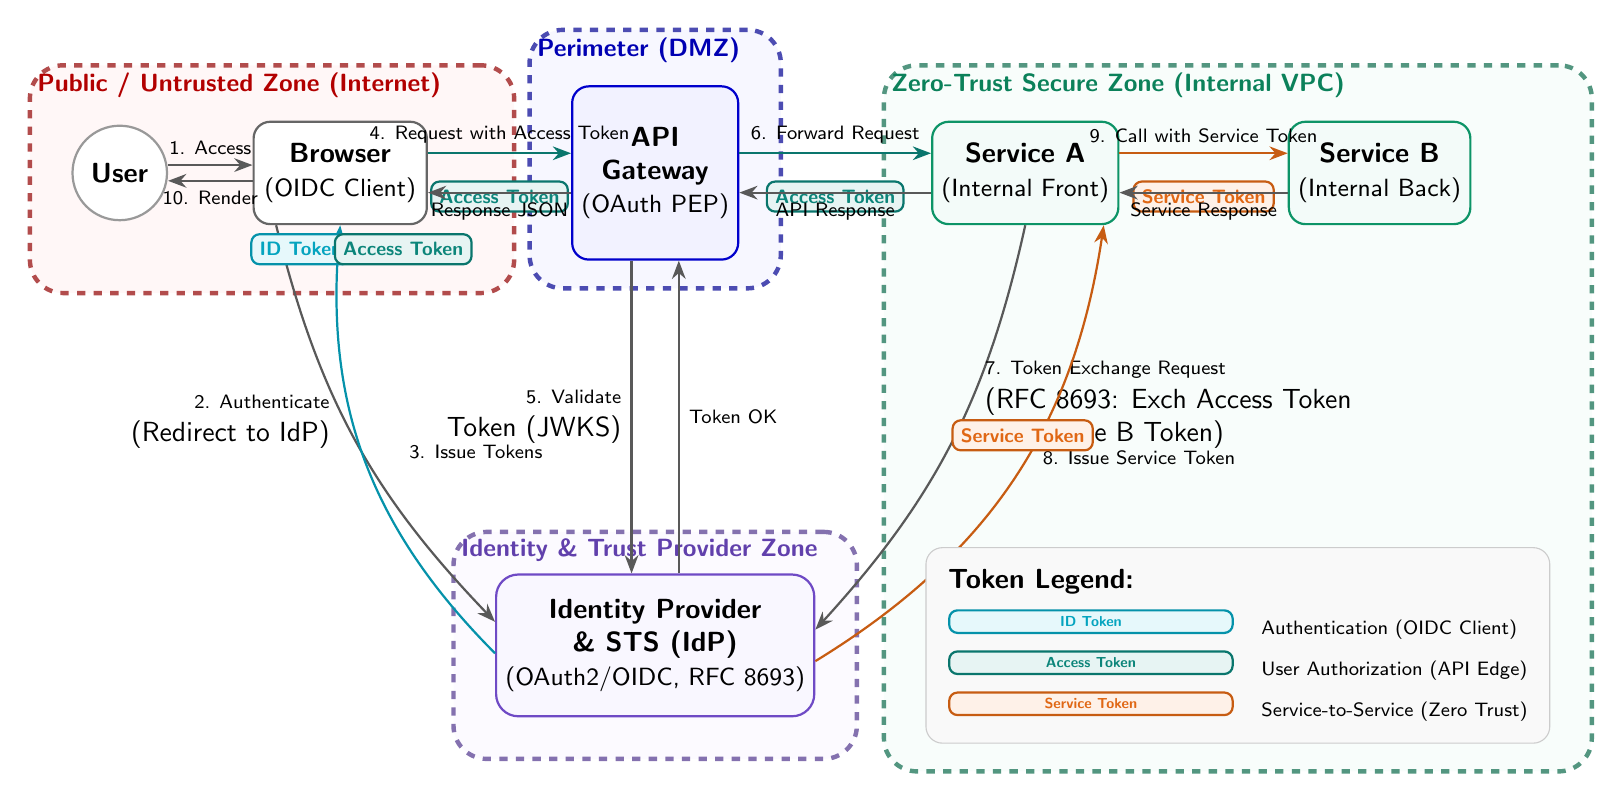
\begin{tikzpicture}[
    font=\sffamily,
    >=Stealth,
    node distance=1.5cm and 2cm,
    % Colors
    every node/.style={color=black},
    % Styles
    box/.style={
        draw, rectangle, rounded corners=6pt, 
        minimum height=1.3cm, minimum width=2.2cm, 
        align=center, fill=white, thick,
        draw=blue!80!black
    },
    actor/.style={
        draw, circle, minimum size=1.2cm, 
        fill=white, thick, draw=gray!80,
        align=center
    },
    gateway/.style={
        draw, rectangle, rounded corners=6pt,
        minimum height=2.2cm, minimum width=1.5cm,
        fill=blue!5!white, thick, draw=blue!80!black,
        align=center
    },
    idp/.style={
        draw, rectangle, rounded corners=8pt,
        minimum height=1.8cm, minimum width=3.8cm,
        fill=purple!5!white, thick, draw=purple!80!black,
        align=center
    },
    token/.style={
        draw, rectangle, rounded corners=3pt,
        font=\scriptsize\sffamily\bfseries,
        inner sep=3pt,
        align=center,
        thick
    },
    idtoken/.style={token, fill=cyan!10, draw=cyan!80!black, text=cyan!90!black},
    acctoken/.style={token, fill=teal!10, draw=teal!80!black, text=teal!90!black},
    svctoken/.style={token, fill=orange!10, draw=orange!80!black, text=orange!90!black},
    % Flow arrows
    flow/.style={
        ->, thick, draw=gray!70!black
    },
    tokenflow/.style={
        ->, dashed, thick, draw=blue!70!black
    },
    stepnum/.style={
        draw, circle, fill=black, text=white,
        font=\scriptsize\bfseries, inner sep=1pt,
        minimum size=4.5mm, align=center
    }
]

% Define modern colors
\definecolor{emerald}{HTML}{10B981}
\definecolor{cyan}{HTML}{06B6D4}
\definecolor{teal}{HTML}{0D9488}
\definecolor{orange}{HTML}{F97316}
\definecolor{purple}{HTML}{8B5CF6}
\definecolor{darkgray}{HTML}{4B5563}

% ==================== NODES ====================

% Coordinates for clean layout
\coordinate (user_pos) at (0, 3.5);
\coordinate (browser_pos) at (2.8, 3.5);
\coordinate (gw_pos) at (6.8, 3.5);
\coordinate (svca_pos) at (11.5, 3.5);
\coordinate (svcb_pos) at (16.0, 3.5);
\coordinate (idp_pos) at (6.8, -2.5);

% Nodes placement
\node (user) [actor] at (user_pos) {\textbf{User}};
\node (browser) [box, draw=gray!80!black, fill=white] at (browser_pos) {\textbf{Browser}\\\small (OIDC Client)};
\node (gw) [gateway] at (gw_pos) {\textbf{API}\\\textbf{Gateway}\\\small(OAuth PEP)};
\node (svca) [box, draw=emerald!80!black, fill=emerald!5!white] at (svca_pos) {\textbf{Service A}\\\small(Internal Front)};
\node (svcb) [box, draw=emerald!80!black, fill=emerald!5!white] at (svcb_pos) {\textbf{Service B}\\\small(Internal Back)};
\node (idp) [idp] at (idp_pos) {\textbf{Identity Provider}\\\textbf{\& STS (IdP)}\\\small(OAuth2/OIDC, RFC 8693)};

% ==================== FLOWS & ANNOTATIONS ====================

% 1. User -> Browser
\draw[flow] ($(user.east)+(0,0.1)$) -- ($(browser.west)+(0,0.1)$) 
    node[midway, above] {\scriptsize 1. Access};
\draw[flow] ($(browser.west)-(0,0.1)$) -- ($(user.east)-(0,0.1)$) 
    node[midway, below] {\scriptsize 10. Render};

% 2. Browser -> IdP (Auth Request)
\draw[flow] ($(browser.south west)+(0.3,0)$) to[bend right=15] 
    node[pos=0.45, left, xshift=-2pt, align=right] {\scriptsize 2. Authenticate\\(Redirect to IdP)} 
    ($(idp.west)+(0,0.3)$);

% 3. IdP -> Browser (Tokens)
\draw[flow, draw=cyan!80!black] ($(idp.west)+(0,-0.1)$) to[bend left=25] 
    node[pos=0.55, right, xshift=15pt, yshift=-5pt, align=left] (tokens_lbl) {\scriptsize 3. Issue Tokens}
    ($(browser.south)+(0,0)$);
% Token badges for Step 3
\node (id_token_3) [idtoken, below=0.1cm of browser, xshift=-0.5cm] {ID Token};
\node (acc_token_3) [acctoken, below=0.1cm of browser, xshift=0.8cm] {Access Token};

% 4. Browser -> API Gateway
\draw[flow, draw=teal!80!black] ($(browser.east)+(0,0.25)$) -- ($(gw.west)+(0,0.25)$)
    node[midway, above] {\scriptsize 4. Request with Access Token};
\node (acc_token_4) [acctoken] at ($(browser.east)!0.5!(gw.west)+(0,-0.3)$) {Access Token};

% 5. API Gateway -> IdP (Validate Token) - Parallel vertical lines
\draw[flow] ($(gw.south)-(0.3,0)$) -- ($(idp.north)-(0.3,0)$)
    node[midway, left, align=right] {\scriptsize 5. Validate\\Token (JWKS)};
\draw[flow] ($(idp.north)+(0.3,0)$) -- ($(gw.south)+(0.3,0)$)
    node[midway, right] {\scriptsize Token OK};

% 6. API Gateway -> Service A
\draw[flow, draw=teal!80!black] ($(gw.east)+(0,0.25)$) -- ($(svca.west)+(0,0.25)$)
    node[midway, above] {\scriptsize 6. Forward Request};
\node (acc_token_6) [acctoken] at ($(gw.east)!0.5!(svca.west)+(0,-0.3)$) {Access Token};

% 7. Service A -> IdP (Token Exchange)
\draw[flow] ($(svca.south)+(0,0)$) to[bend left=15]
    node[pos=0.4, right, xshift=2pt, align=left] {\scriptsize 7. Token Exchange Request\\(RFC 8693: Exch Access Token\\for Service B Token)}
    ($(idp.east)+(0,0.2)$);

% 8. IdP -> Service A (Service Token)
\draw[flow, draw=orange!80!black] ($(idp.east)+(0,-0.2)$) to[bend right=25]
    node[pos=0.55, right, xshift=2pt, align=left] {\scriptsize 8. Issue Service Token}
    ($(svca.south east)-(0.2,0)$);
\node (svc_token_8) [svctoken] at ($(idp.east)!0.5!(svca.south)+(1.3,0)$) {Service Token};

% 9. Service A -> Service B
\draw[flow, draw=orange!80!black] ($(svca.east)+(0,0.25)$) -- ($(svcb.west)+(0,0.25)$)
    node[midway, above] {\scriptsize 9. Call with Service Token};
\node (svc_token_9) [svctoken] at ($(svca.east)!0.5!(svcb.west)+(0,-0.3)$) {Service Token};

\draw[flow] ($(svcb.west)-(0,0.25)$) -- ($(svca.east)-(0,0.25)$)
    node[midway, below] {\scriptsize Service Response};

% Responses returning
\draw[flow] ($(svca.west)-(0,0.25)$) -- ($(gw.east)-(0,0.25)$)
    node[midway, below] {\scriptsize API Response};

\draw[flow] ($(gw.west)-(0,0.25)$) -- ($(browser.east)-(0,0.25)$)
    node[midway, below] {\scriptsize Response JSON};

% ==================== LEGEND ====================
\node (legend) [
    draw=gray!40, rectangle, rounded corners=6pt, fill=gray!5, 
    minimum width=4.8cm, align=left, inner sep=8pt
] at (14.2, -2.5) {
    \textbf{Token Legend:}\\[1.5mm]
    \tikz\node[idtoken, scale=0.75]{ID Token}; \ \ {\scriptsize Authentication (OIDC Client)}\\[1mm]
    \tikz\node[acctoken, scale=0.75]{Access Token}; \ \ {\scriptsize User Authorization (API Edge)}\\[1mm]
    \tikz\node[svctoken, scale=0.75]{Service Token}; \ \ {\scriptsize Service-to-Service (Zero Trust)}
};

% ==================== BACKGROUND / ZONES ====================

\begin{pgfonlayer}{background}
    % Public Zone
    \node (public_zone) [
        draw=red!40!gray, fill=red!3!white, dashed, ultra thick, rounded corners=12pt,
        fit=(user) (browser) (id_token_3) (acc_token_3),
        inner sep=15pt, yshift=5pt
    ] {};
    \node[anchor=north west, font=\bfseries\sffamily\small, text=red!70!black] at (public_zone.north west) {Public / Untrusted Zone (Internet)};

    % DMZ Zone
    \node (dmz_zone) [
        draw=blue!40!gray, fill=blue!3!white, dashed, ultra thick, rounded corners=12pt,
        fit=(gw),
        inner sep=15pt, yshift=5pt
    ] {};
    \node[anchor=north west, font=\bfseries\sffamily\small, text=blue!70!black] at (dmz_zone.north west) {Perimeter (DMZ)};

    % Zero Trust Secure Zone
    \node (secure_zone) [
        draw=emerald!40!gray, fill=emerald!3!white, dashed, ultra thick, rounded corners=12pt,
        fit=(svca) (svcb) (svc_token_9) (legend),
        inner sep=15pt, yshift=5pt
    ] {};
    \node[anchor=north west, font=\bfseries\sffamily\small, text=emerald!70!black] at (secure_zone.north west) {Zero-Trust Secure Zone (Internal VPC)};

    % IdP / Trust Zone
    \node (idp_zone) [
        draw=purple!40!gray, fill=purple!3!white, dashed, ultra thick, rounded corners=12pt,
        fit=(idp),
        inner sep=15pt
    ] {};
    \node[anchor=north west, font=\bfseries\sffamily\small, text=purple!70!black] at (idp_zone.north west) {Identity \& Trust Provider Zone};
\end{pgfonlayer}

\end{tikzpicture}
\end{document}
